\documentclass{icga}
\usepackage{graphicx}
\def\Dx{\mbox{\sc DeepHex}}
\def\Eo{\mbox{\sc Ezo}}
\def\Mx{\mbox{\sc MoHex}}
\def\Sol{\mbox{\sc Solver}}
\def\Fuego{\mbox{\sc Fuego}}
\def\TV{\mbox{\sc TV}} %Tony van der Valk

\title{\sc MOHEX WINS 2015 HEX 11x11 and HEX 13x13 TOURNAMENTS}
\runningtitle{ICGA}
\author{Ryan Hayward\thanks{Department 
of Computing Science, University of Alberta, Canada. Email:hayward@ualberta.ca} and
Jakub Pawlewicz\thanks{Institute of Informatics, University of Warsaw, Poland. Email:pan@mimuw.edu.pl} and
Kei Takada\thanks{Hokkaido University, Japan. Email:takada@complex.ist.hokudai.ac.jp} and
Tony van der Valk\thanks{Email:tony@hexboard.com}
}
\affiliation{Edmonton, Canada}
\issue{Volume 39 (2017) IOS Press 60-64}

\setcounter{page}{60}
\begin{document}
\maketitle

\vspace*{-2.25in}
%{\it ICGA Journal Vol.\ XX No.\ YY Sept 999 pp ??-??
%\hfill Computer Games Olympiad, 2015 Leiden.}
%{\it ICGA Journal 39 (2017) 60-64}
\vspace*{2.0in}

\begin{figure}[hbt]
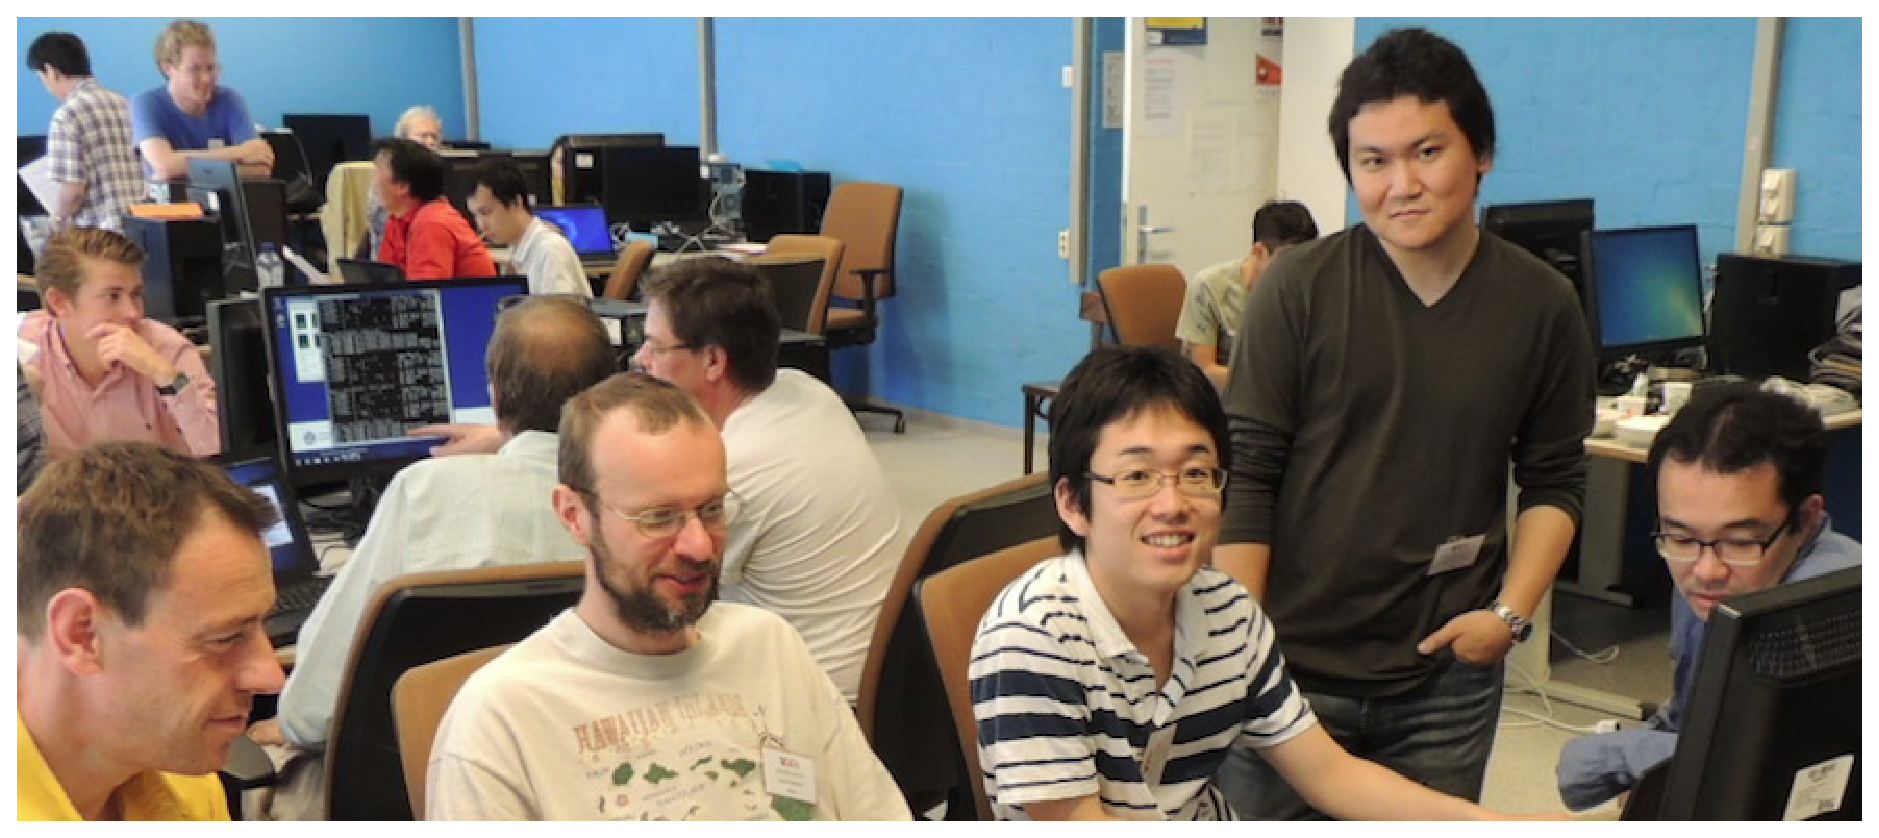
\includegraphics[width=225pt]{edo0.eps}\
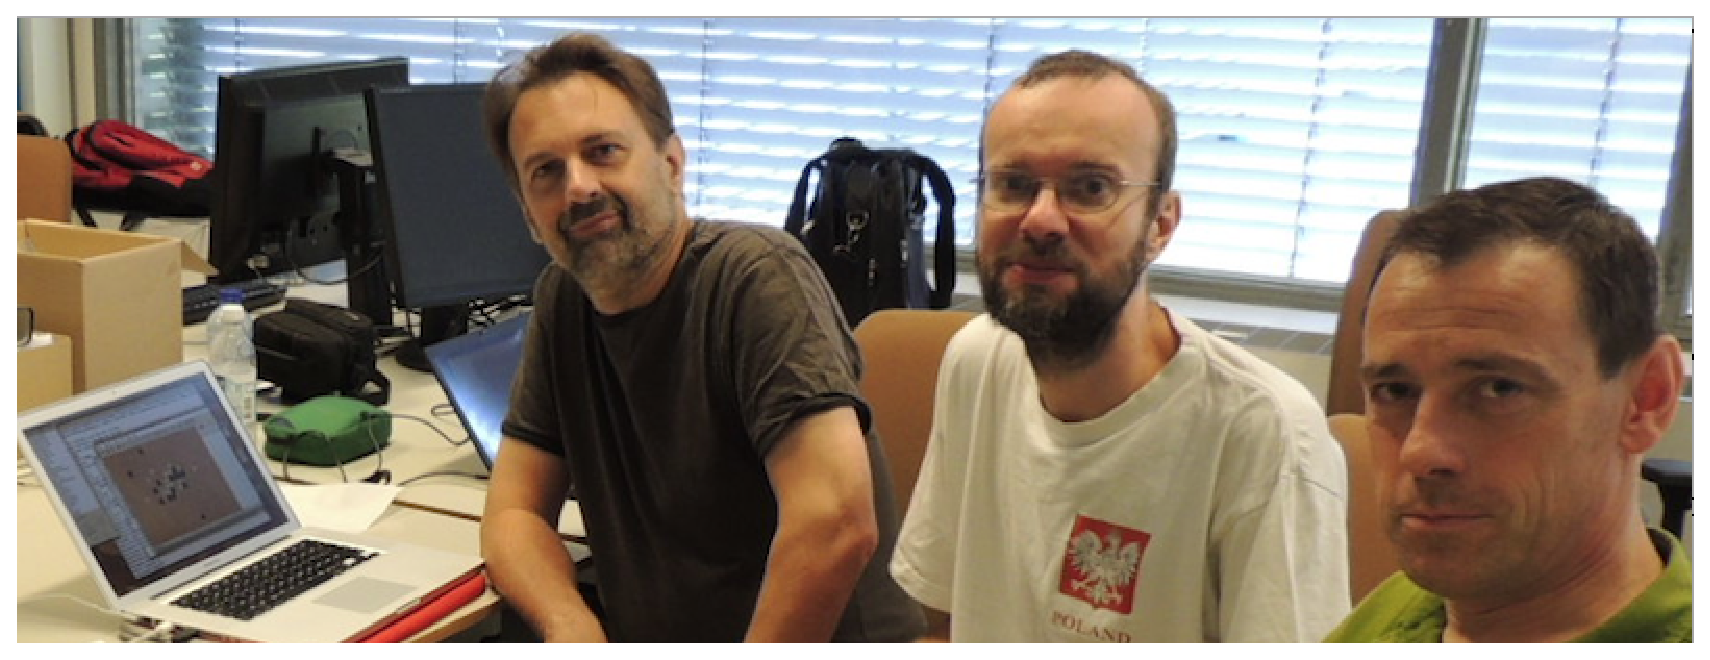
\includegraphics[width=225pt]{rjt2.eps}\\

\hfill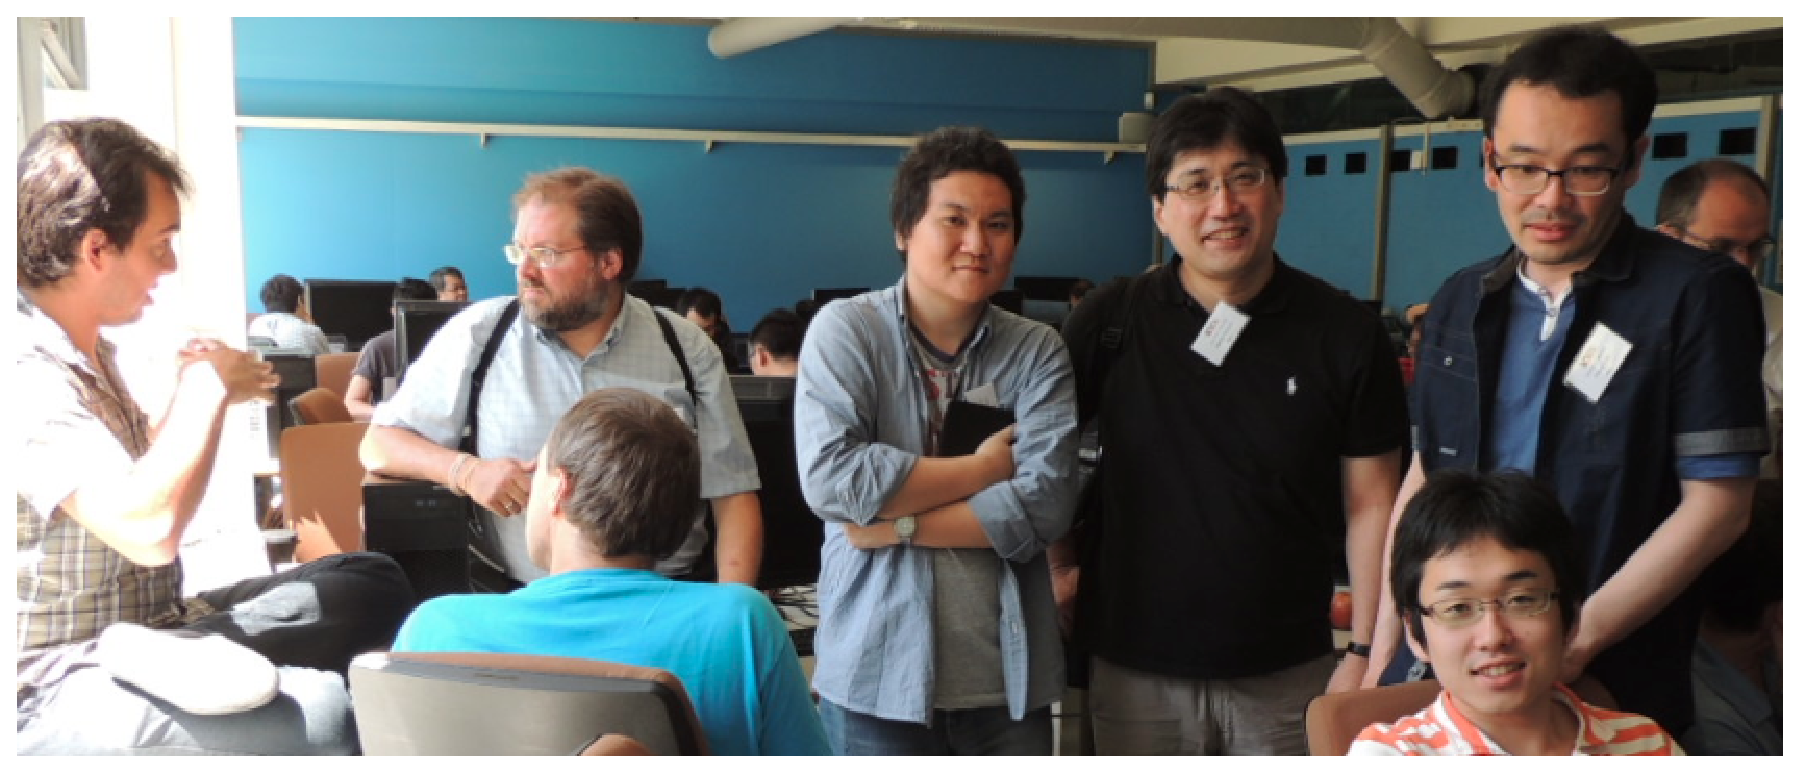
\includegraphics[width=280pt]{mas.eps}\hfill~
\caption{Participants and observers at the Hex competitions.}
\end{figure}


\section{The Tournaments}
At the 2015 Olympiad there were
two Hex tournaments: 11$\times$11 and 13$\times$13.
Three programs competed in each tournament:
\Eo{} 
by Kei Takada, supervised by Masahito Yamamoto, from Japan;
\Mx{} 2.0 \citebay{HAHMP13}, 
by Broderick Arneson, Ryan Hayward, Philip Henderson, Aja Huang, and Jakub Pawlewicz,
from Canada;
and
\Dx{}
by Jakub Pawlewicz, 
from Poland.

\Eo{} is a stronger version of the program that competed in the 2013 Olympiad.
\Eo{} uses alpha-beta search with an evaluation function based on
a weighted combination of two different network connectivity measures.
\Eo{} ran on an i7 laptop.

\Dx{} is a new program based on 
Sibling Conspiracy Number Search \citebay{PH15,PH15socs}.
\Dx{}, like \Mx, is based on the Benzene framework, 
developed by Broderick Arneson, Philip Henderson, Ryan Hayward,
Aja Huang, and Jakub Pawlewicz.
\Dx{} ran on a 16 core shared-memory machine.
As an opening book, \Dx{} cached its evaluation scores in a database,
running for 24 hours on each possible opening.

\Mx{}, the winner of the previous four Olympiad Hex competitions
\citebay{HAHP13},
is an MCTS program that uses the Benzene Hex framework
built on the code base of \Fuego\ \citebay{fuego},
the Go program developed by Martin M\"{u}ller, Markus Enzenberger
and others at the University of Alberta.
Benzene allows virtual connection and
inferior cell computations.
\Mx{} performs these computations in UCT tree nodes visited at least 256 times.
\Mx{} ran on a 24 core shared-memory machine, 
with 4 cores reserved for the 
Depth-First Proof Number Search solver, which
produces perfect play if it solves the
position within the time allotted for a move.
\Mx{} uses a book ---
built by Broderick Arneson using Thomas Lincke's method 
\citebay{DBLP:conf/cg/Lincke00} ---
with two 11$\times$11 openings and one 13$\times$13 opening.

Each tournament was a three-player double round robin, so 12 games
in total with 8 games per player.
Post-game win-detection is by our solver.
%Tony van der Walk contributed to this commentary.

{\large\bf 11$\times$11 Tournament}

\hfill\begin{tabular}{|c|c|c|c|c|c|}
\hline 11x11 results &\Mx{} &\Dx{}    & \Eo{}     & total & result \\ 
\hline \Mx{} &      &  3-1    &  4-0      & 7-1  & gold \\
\hline \Dx{} &  1-3 &         &  4-0      & 5-3  &  silver\\
\hline \Eo{} &  0-4 &  0-4    &           & 0-8  &  bronze \\
\hline
\end{tabular}\hfill~

Here are some selected games.

{\bf Game 1.}
%{\sc \Eo-\Mx\ 0-1.}
{\sc E-M 0-1.}
1.B[a7] 2.W[swap] 3.W[c9] \ldots ~ ~
\Mx{} sees the win by move 30.B[e4].

{\bf Game 2.}
%{\sc \Dx-\Eo\ 1-0.}
{\sc D-E 1-0.}
1.B[a3] 2.W[c9] \ldots ~ ~
\Eo{} opens well, but blunders: 28.W[h2] wins.

%{\bf Game 3.}
%{\sc \Mx-\Dx\ 1-0.}
%{\sc M-D 1-0.}
%1.B[a2] 2.W[swap] 3.W[a6] \ldots \ \ 
%\hfill\Mx\ scores increases steadily. Move 19 wins.

%{\bf Game 4.}
%{\sc \Mx-\Eo\ 1-0.}
%{\sc M-E 1-0.}
%1.B[a2] 2.W[j2] 3.B[g6] \ldots \ \ 
%\hfill\Mx{} is happy with \Eo{}'s row 2 ladder. Move 17 wins.

{\bf Game 5.}
%{\sc \Eo-\Dx\ 0-1.}
{\sc E-D 0-1.}
1.B[k5] 2.W[swap] 3.W[i3] \ldots ~ ~ 
\Eo{} plays 27.W[i4] instead of j8 or other options that look safer. \Dx{} sees that 28.B[k2] wins.

%{\bf Game 6.}
%{\sc \Dx-\Mx\ 1-0.}
%{\sc D-M 1-0.}
%1.B[g2] 2.W[swap] 3.W[e4] \ldots \ \ 
%\hfill\Mx\ is never comfortable. 23.W[c9] wins.

%{\bf Game 7.}
%{\sc \Eo-\Mx\ 0-1.}
%{\sc E-M 0-1.}
%1.B[f10] 2.W[swap] 3.W[f6] \ldots \ \ 
%\hfill Move 16 wins.

%{\bf Game 8.}
%{\sc \Dx-\Eo\ 1-0.}
%{\sc D-E 1-0.}
%1.B[f2] 2.W[d6] 3.W[e6] \ldots \ \ 
%\hfill Move 13 wins.

{\bf Game 9.}
%{\sc \Mx-\Dx\ 1-0.}
{\sc M-D 1-0.}
1.B[a6] 2.W[swap] 3.W[g5] \ldots ~ ~ 
At move 22, \Dx{} hesitates between j5, which loses, and i8,
which leads to complicated positions where \Mx{} cannot 
find correct moves. But \Dx{} plays 22.B[j5]. Move 30 wins.

%{\bf Game 10.}
%{\sc \Mx-\Eo\ 1-0.}
%{\sc M-E 1-0.}
%1.B[a6] 2.W[c9] 3.W[g7] \ldots \ \ 
%\hfill Move 26 wins.

%{\bf Game 11.}
%%{\sc \Eo-\Dx\ 0-1.}
%{\sc E-D 0-1.}
%1.B[e10] 2.W[g8] 3.W[f8] \ldots \ \ 
%\hfill Move 25 wins.

%{\bf Game 12.}
%%{\sc \Dx-\Mx\ 0-1.}
%{\sc D-M 0-1.}
%1.B[e2] 2.W[f6] 3.B[c8] \ldots \ \ 
%\hfill\Dx{} is never comfortable. Move 13 wins.

\begin{figure}[hbp]

\includegraphics[scale=1.3]{1e-m.eps}\hspace*{-1cm}
\includegraphics[scale=1.3]{2d-e.eps}
\caption{Game 1: \Eo-\Mx\ 0-1. Game 2: \Dx-\Eo\ 1-0.}
\end{figure}

\begin{figure}[hbp]
\includegraphics[scale=1.3]{5e-d.swap.eps}\hspace*{-1cm}\
\includegraphics[scale=1.3]{9m-d.eps}
\caption{Game 5: \Eo-\Dx\ 0-1. Game 9: \Mx-\Dx\ 1-0.}
\end{figure}

\newpage
{\large\bf 13$\times$13 Tournament}


\hfill\begin{tabular}{|c|c|c|c|c|c|}
\hline 13x13 results &\Mx{} &\Dx{}         & \Eo{}     & total & result \\ 
\hline \Mx{} &      &  2-2 (2-0)   &  4-0      & 6-2  (2-0) & gold \\
\hline \Dx{} &  2-2 (0-2) &         &  4-0      & 6-2 (0-2) &  silver\\
\hline \Eo{} &  0-4 &  0-4    &           & 0-8  &  bronze \\
\hline
\end{tabular}\hfill~

Above, playoff results are inside parentheses.
Here are some selected games.
%{\bf Game 1.}
%%{\sc \Eo-\Mx\ 0-1.}
%{\sc E-M 0-1.}
%1.B[a8] 2.W[swap] 3.W[b12] \ldots \ \ 
%\hfill Move 30 wins.

%{\bf Game 2.}
%{\sc \Dx-\Eo\ 1-0.}
%{\sc D-E 1-0.}
%1.B[a10] 2.W[l2] 3.B[j3] \ldots \ \ 
%\hfill Move 31 wins.

{\bf Game 3.}
%{\sc \Mx-\Dx\ 1-0.}
{\sc M-D 1-0.}
1.B[a7] 2.W[swap] 3.W[i5] \ldots ~ ~
For many moves, both programs see this game as even.
\Mx\ turns the corner with move 29, 
not seeing how to use i5 to connect to the right side.
45.W[g4] is unexpected, but wins.
This game shows the importance of virtual connections and
an endgame solver.

%{\bf Game 4.}
%{\sc \Mx-\Eo\ 1-0.}
%{\sc M-E 1-0.}
%1.B[a7] 2.W[c11] 3.B[i8] \ldots \ \ 
%\hfill\Mx{} finds a win by 35.B[h3].

%{\bf Game 5.}
%%{\sc \Eo-\Dx\ 0-1.}
%{\sc E-D 0-1.}
%1.B[m3] 2.W[swap] 3.W[l2] \ldots \ \ 
%28.W[f2] looks reasonable, but is out of the mustplay
%region computed by Benzene's virtual connection engine,
%so \Dx\ finds a win with the next move.

{\bf Game 6.}
%{\sc \Dx-\Mx\ 1-0.}
{\sc D-M 1-0.}
1.B[j2] 2.W[g8] 3.W[d10] \ldots ~ ~
A close game. 
\Mx\ blunders with 54.W[f9]; 54.W[l11] wins.
\Dx\ sees the win soon after.

%{\bf Game 7.}
%{\sc \Eo-\Mx\ 0-1.}
%{\sc E-M 0-1.}
%1.B[m8] 2.W[f8] 3.B[b12] \ldots \ \ 
%\hfill\Mx\ sees the win by move 38.

%{\bf Game 8.}
%%{\sc \Dx-\Eo\ 1-0.}
%{\sc D-E 1-0.}
%1.B[a11] 2.W[b12] 3.B[c11] \ldots \ \ 
%\Eo{} looks behind early, \Dx\ sees a win by move 23.

%{\bf Game 9.}
%{\sc \Mx-\Dx\ 1-0.}
%{\sc M-D 1-0.}
%1.B[a7] 2.W[swap] 3.W[i5] \ldots \ \ 
%
%\hfill The same opening as Game 3.
%Non-deterministic \Mx\ plays differently from move 5.
%Move 33 wins.
%
%{\bf Game 10.}
%%{\sc \Mx-\Eo\ 1-0.}
%{\sc M-E 1-0.}
%1.B[a7] 2.W[c11] 3.W[i8] \ldots \ \ 
%
%\hfill\Mx\ score jumps after 10.W[g12] (expected k3)
%and after 24.W[j3]. \Mx\ sees the win by move 27.

{\bf Game 11.}
%{\sc \Eo-\Dx\ 0-1.}
{\sc E-D 0-1.}
1.B[a4] 2.W[swap] 3.W[k3] \ldots ~ ~ 
A close game. From move 20, \Dx\ behaves unexpectedly,
perhaps because its move selection does not consider inferior cells:
move 28 considers neither a3 nor f2 (which captures a3).
Here \Mx\ likes f2, but \Dx\ plays k4.
\Eo\ then takes a3, and gets into a winning position:
47.W[k11] wins, although this takes the solver a long time to check.
But \Eo\ plays 47.W[j10] and \Dx\ grinds out a win.

%{\bf Game 12.}
%{\sc \Dx-\Mx\ 0-1.}
%{\sc D-M 0-1.}
%1.B[d2] 2.W[e9] 3.B[g8] \ldots \ \ 
%\hfill\Mx\ never looks comfortable. Move 35 wins.

{\bf Playoff Game 1.}
%{\sc \Mx-\Dx\ 1-0.}
{\sc M-D 1-0.}
1.B[a7] 2.W[h12] 3.B[c11] \ldots \ \ 
Earlier \Dx\ swapped and lost, so here not-swaps.
\Mx\ scores increase gradually. Move 46 wins.

%{\bf Playoff Game 2.}
%{\sc \Dx-\Mx\ 0-1.}
%{\sc D-M 0-1.}
%1.B[j2] 2.W[swap] 3.W[d3] \ldots \ \ 
%Earlier \Mx\ not-swapped and lost, so here swaps. 
%No stones touch until move 14. \Mx\ sees a win by move 24.

\begin{figure}[hbp]
\includegraphics[scale=1.3]{13.03m-d.swap.eps}\hspace*{-2.5cm}\
\includegraphics[scale=1.3]{13.06d-m.eps}
\caption{Game 3: \Mx-\Dx\ 1-0. ~ ~ Game 6: \Dx-\Mx\ 1-0.}
\end{figure}

\begin{figure}[hbp]
\includegraphics[scale=1.3]{13.11e-d.swap.eps}\hspace*{-2.5cm}\
\includegraphics[scale=1.3]{13.p01m-d.eps}
\caption{Game 11: \Eo-\Dx\ 0-1. ~ ~ Playoff Game 1: \Mx-\Dx\ 1-0.}
\end{figure}

\newpage
{\large\bf Man-Machine Exhibition} 

An informal man-machine exhibition took place after the tournaments:
Tony van der Valk (\TV), ranked 5th-ranked in Hex on Little Golem,
played two games --- 11$\times$11, 15m/player --- 
each against \Dx\ and \Mx. The machines won all four games.
Below we show two of these games.

%{\bf Game 1.}
%%{\sc \Mx-\TV\ 1-0.}
%{\sc M-T 1-0.}
%1.B[a2] 2.W[swap] 3.W[f6] \ldots \hfill Move 23 wins.

%{\bf Game 2.}
%%{\sc \TV-\Mx\ 0-1.}
%{\sc T-M 0-1.}
%1.B[f2] 2.W[e7] 3.B[c8] \ldots \hfill Move 16 wins.

%{\bf Game 3.}
%{\sc \Dx-\TV\ 1-0.}
%{\sc D-T 1-0.}
%1.B[g2] 2.W[f4] 3.B[h5] \ldots \hfill Move 15 wins.

%{\bf Human-compter exhibition Game 4.}
%{\sc \TV-\Dx\ 0-1.}
%{\sc T-D 0-1.}
\begin{figure}[hbp]
%1.B[f2] 2.W[h9] 3.B[f9] \ldots \hfill Move 24 wins.
\includegraphics[scale=1.3]{m-tony.swap.eps}\hspace*{-2cm}\
\includegraphics[scale=1.3]{tony-d.eps}
\caption{\Mx-\TV\ 1-0. ~ ~ \TV-\Dx\ 0-1.}
\end{figure}

\section{Conclusions}
%{\large\bf Conclusions}
\Eo{}'s performance was stronger than its record indicates. 
It played some strong openings and had winning moves deep
into games against \Dx.
It was unlucky not to win a game.

\Dx\ and \Mx\ were evenly matched, but play different styles.
\Mx\ seems stronger in opening and early middle play,
but its Monte Carlo simulations cannot handle tactical positions.
\Dx\ thrives on tactical positions, and is especially
strong in the late middle game in complicated positions.

{\bf Acknowledgements.}
We thank the NSERC Discovery Grant Program for research funding,
Martin M\"{u}ller for the loan his machine,
and Philip Henderson for comments on a draft of this report.
\bibliography{rpt}

%\includegraphics[scale=1.3]{3m-d.eps}\hspace*{-1cm}\includegraphics[scale=1.3]{4m-e.eps}

%{\bf 11$\times$11: Games 1-4 (top left/right, bottom left/right).}
%\Eo-\Mx\ 0-1, \Dx-\Eo\ 1-0, \Mx-\Dx\ 0-1, \Mx-\Eo\ 1-0.

%\includegraphics[scale=1.3]{5e-d.swap.eps}\hspace*{-1cm}
\includegraphics[scale=1.3]{6d-m.eps}

%\includegraphics[scale=1.3]{7e-m.eps}\hspace*{-1cm}\includegraphics[scale=1.3]{8d-e.eps}

%\includegraphics[scale=1.3]{9m-d.eps}\hspace*{-1cm}\includegraphics[scale=1.3]{10m-e.eps}

%\includegraphics[scale=1.3]{11e-d.eps}\hspace*{-1cm}\includegraphics[scale=1.3]{12d-m.eps}

%{\bf 11$\times$11: Games 5-12.}

%\newpage
%\includegraphics[scale=1.3]{13.01e-m.swap.eps}\hspace*{-2.5cm}\includegraphics[scale=1.3]{13.02d-e.eps}

%\includegraphics[scale=1.3]{13.03m-d.swap.eps}\hspace*{-2.5cm}\includegraphics[scale=1.3]{13.04m-e.eps}

%\includegraphics[scale=1.3]{13.05e-d.swap.eps}\hspace*{-2.5cm}\includegraphics[scale=1.3]{13.06d-m.eps}

%\includegraphics[scale=1.3]{13.07e-m.eps}\hspace*{-2.5cm}\includegraphics[scale=1.3]{13.08d-e.eps}

%\includegraphics[scale=1.3]{13.09m-d.swap.eps}\hspace*{-2.5cm}\includegraphics[scale=1.3]{13.10m-e.eps}

%\includegraphics[scale=1.3]{13.11e-d.swap.eps}\hspace*{-2.5cm}\includegraphics[scale=1.3]{13.12d-m.eps}

%{\bf 13$\times$13: Games 1-12.}

%\ 

%\includegraphics[scale=1.3]{13.p01m-d.eps}\hspace*{-2.5cm}\includegraphics[scale=1.3]{13.p02d-m.swap.eps}

%{\bf 13$\times$13: Playoff games. \Mx-\Dx\ 1-0, \Dx-\Mx\ 0-1.}

%\newpage
%\includegraphics[scale=1.3]{m-tony.swap.eps}\hspace*{-2cm}\includegraphics[scale=1.3]{tony-m.eps}

%\includegraphics[scale=1.3]{d-tony.eps}\hspace*{-2cm}\includegraphics[scale=1.3]{tony-d.eps}

%{\bf Human-computer games. Top: \Mx-\TV\ 1-0, \TV-\Mx\ 0-1.
%Bottom: \Dx-\TV\ 1-0, \TV-\Dx\ 0-1. Each player had 15 minutes to
%make all moves.}
\end{document}
%{\bf Tony comments}
%I just pick a few games to comment upon. Hard to know if my comments are better on a par with the outcome of the programs reasoning. 
%For instance, look at 11x11 game 9m-d. In your comment you state 22 J5 is losing. But in my analysis 22 J5, 23 J6, 24 F9 could well be winning. Do you agree? Does Mohex agree?  
%
%Ryan: no, 25.W[e10] wins.
%
%Next look at 13x13 game 6d-m. 
%"Game 6. DEEPHEX-MOHEX 1-0. 1.B[j2] 2.W[g8] 3.W[d10] . . . Another close game. MOHEX blunders with
%54.W[f9]; 54.W[l11] wins. DEEPHEX sees the win soon after." 
%Move 3 should be B[d10] I presume. 
%Perhaps I do not understand te comments here: at move 66 I13 white seems to be winning after all? So what is wrong with 54 W[f9]? 
%
%ome further notes...
%
%First I see now why Game 13.06d-m was lost. Incredible that the program could find such elaborate moves as W[f9] or W[I11]. 
%But when I go back a little further in the game I wonder about 30 W[b6] which is clearly too early. Human players would always play 30Wb11; 31Ba12; 32Wb12; 33Ba13 first and only then 34Wb6. Next the same sequence may happen at the right side of the board, resulting in the position of the attached game. I think this is a white win. 
%
%Ryan: no, solver finds black wins from this state:
%PV j12 j11 i12 i11 h12 h11 g12 g11 f12 f10 j3 i4 i3 h4 h2 h3 i2 g3 g2 e3 f1 d2 e12 d12 e11 d11 f3 e5 g10 f11 d3 e2
%
%In game 13.11e-d Deephex plays remarkably indeed, discarding the obvious connection at a3. However, after 27Ba3 black would face difficulties connecting the black chain on the left to the bottom. I can see no easy win for white after 27Bk4 as played in the game. In your comment you mention that 47Wk11 would be a win for EZO. However black seems to have opportunities to defend against Wk11, of which my analysis in the attached game presents one example. Other progressions are possible too, but I did not yet find a better answer for white. All in all this game shows to me how very deep Deephex is looking into the game! 
%
%In the first playoff game we see white answering very far to the bottom, playing 2Wh12 instead of a usual (human) move like 2Wi10. Next 6Wc8 seems a weak move. As long as white has at least two options to connect it should postpone connecting and strengthen instead, but if white has only one remaining option it seems better to connect right away. This could result in a better position like in the commented game: 6Wb9; 7Bc9; 8Wd7; until 15Wb5. But of course black may answer differently. 
%"Playoff Game 1. MOHEX-DEEPHEX 1-0. 1.B[a7] 2.W[h12] 3.W[c11] . . . DEEPHEX lost earlier when swapping
%this opening, so here it does not swap. MOHEX scores gradually increased, and finds a win by move 46."
%I guess move three has to be 3.B[c11]? 
%I can see that in the game 47Bj6 is a winning move. 
